
\chapter{Discriminative vs. Generative Models}\label{discriminative_modelinmg}
\section{Overview}
Machine learning models can be classified into two main categories, discriminative and generative models. Simply put, a discriminative model makes predictions based on conditional probability $p\left(y|\bx\right)$ and is used for classification or regression problems. In other words, discriminative models distinguishes the decision boundary between the
classes.  It corresponds to learning parameters that maximize the conditional probability
distribution $p(y|\bx)$. On the contrary, a generative model revolves around the distribution of a data set to return a probability for a given example. Rather than
looking at classes and trying to find something to separate them, it focuses
only on the one class at the time and builds a model what that certain class looks like, then turns attention to the other class. To express it more formally, generative models learn parameters that maximize $p\left(\bx|y \right)$ and $p\left(y\right)$. Since
\begin{align}\label{eq:prob_decompostion}
p\left(\bx,y\right) = p\left(\bx|y\right)\cdot p\left(y\right),
\end{align}
with joint PDF it is possible to generate new $\left(\bx',y'\right)$ pairs. In some cases, the use of the second decomposition $p\left(\bx,y\right) = p\left(y|\bx\right)\cdot p\left(\bx\right)$ is also an option.  Note that in an unsupervised setting, the task is reduced to inferring only $p\left(\bx\right)$.
\begin{figure}[h]
	\centering
	\begin{minipage}{.5\textwidth}
		\centering
		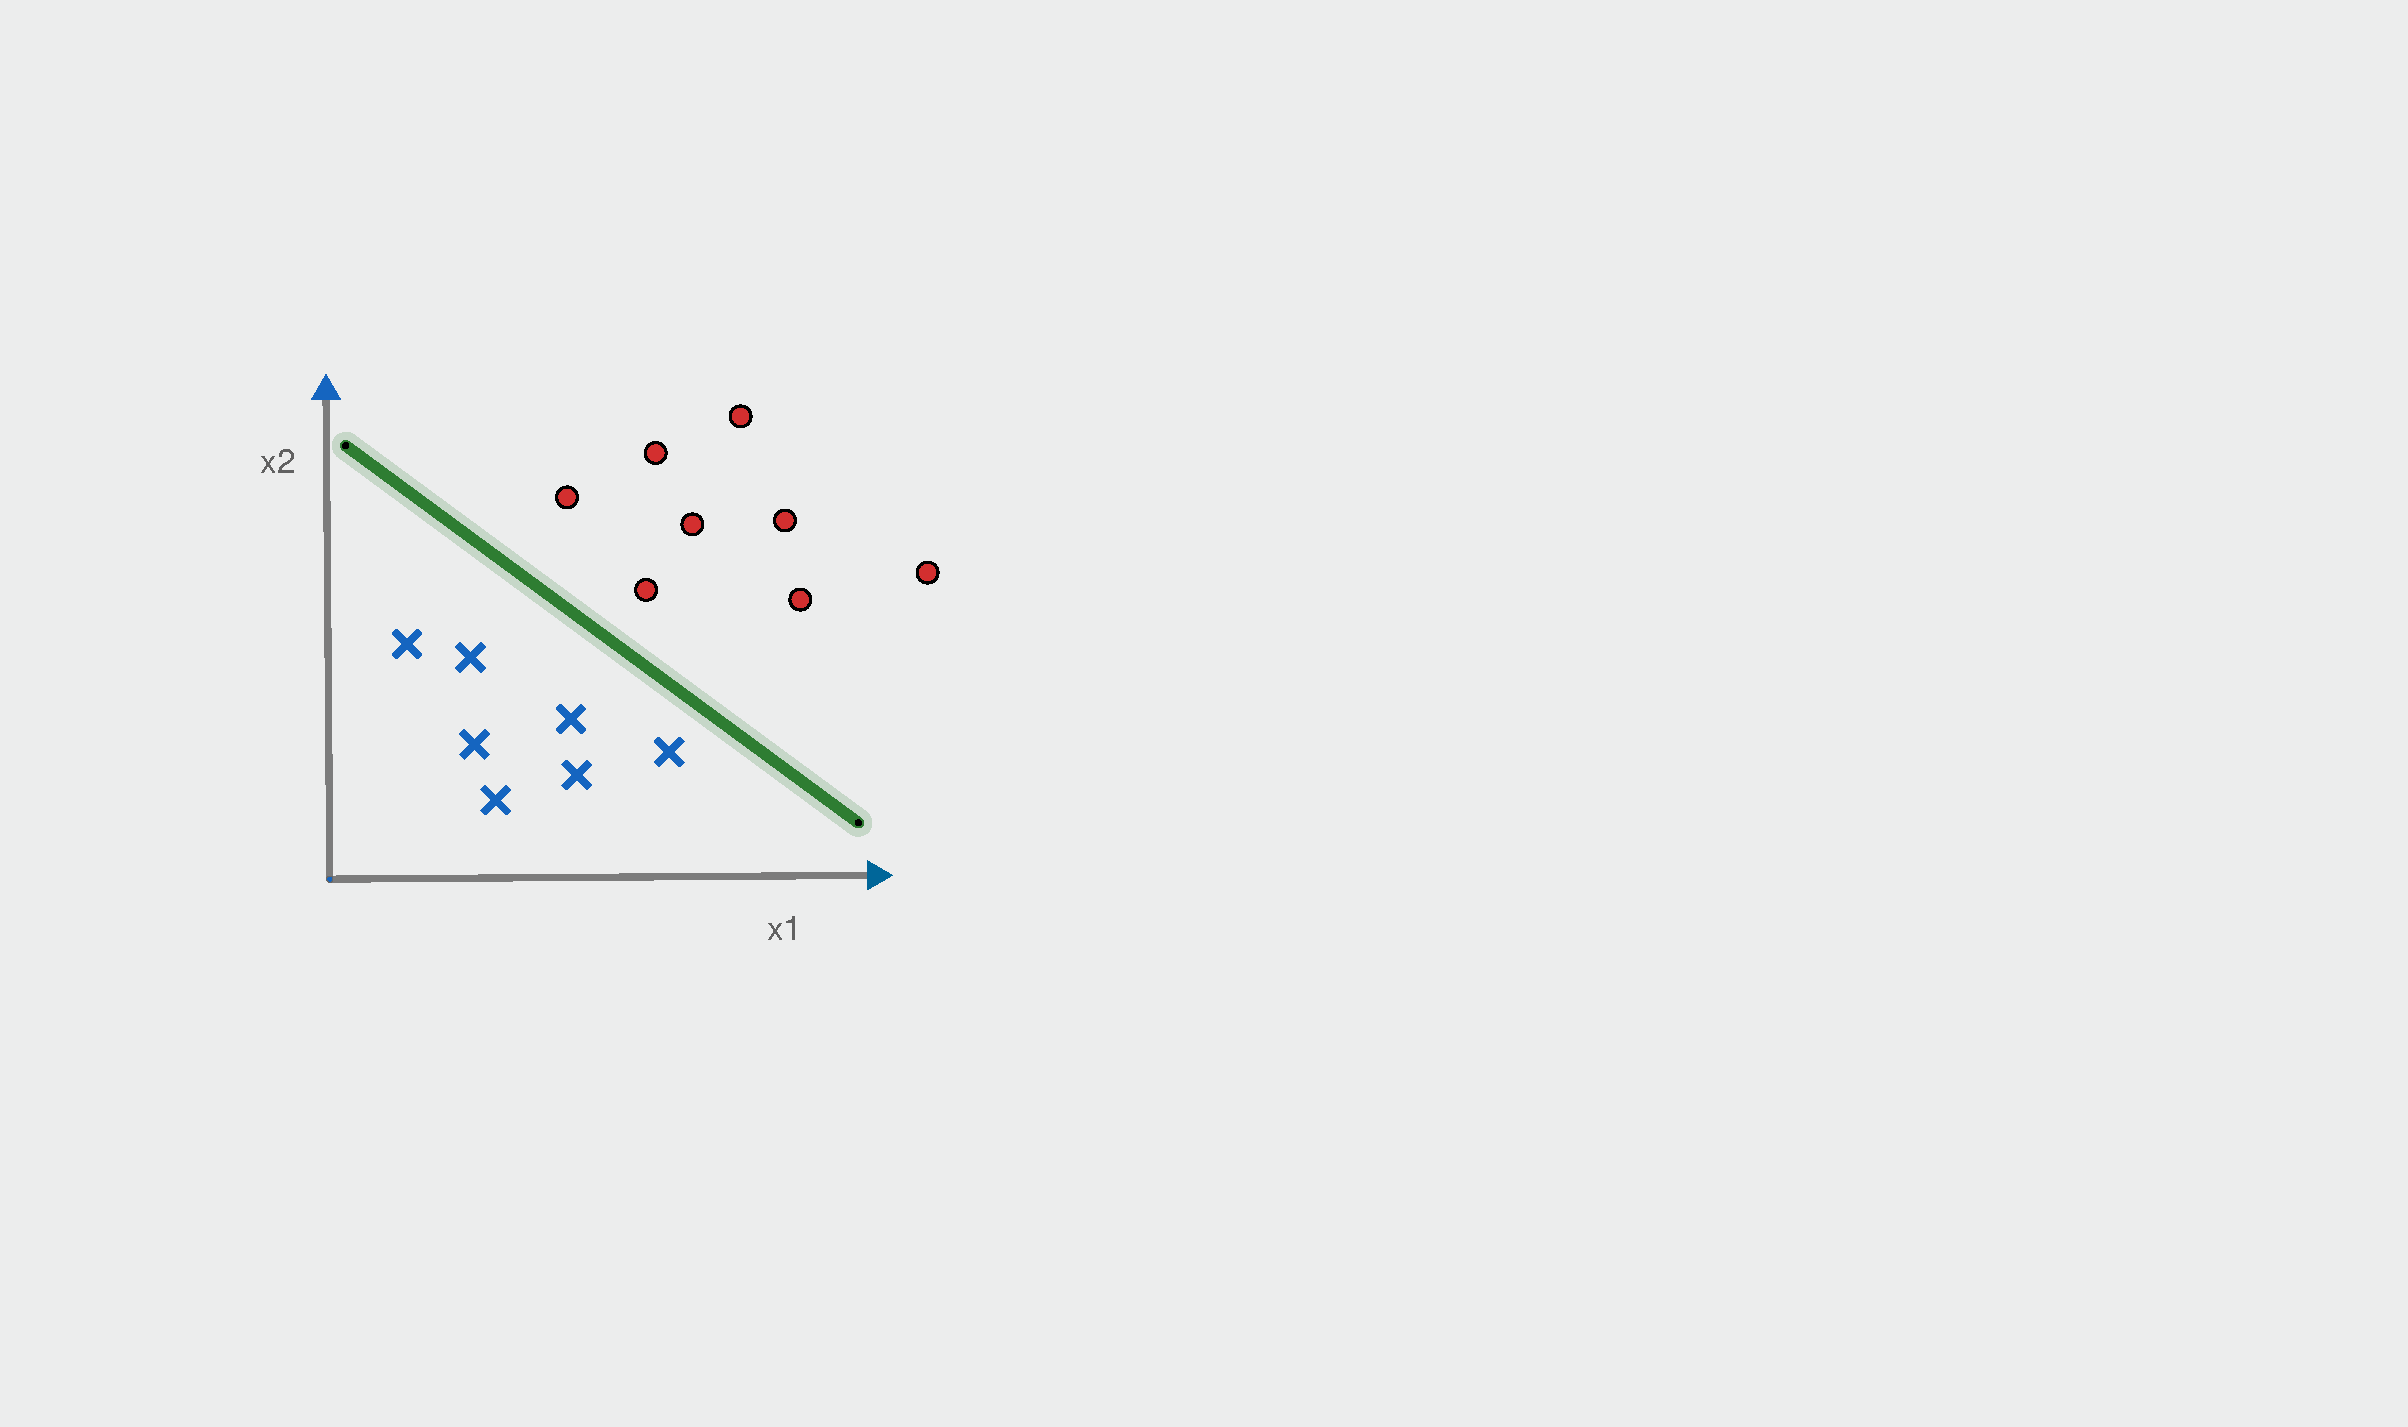
\includegraphics[trim = 4cm 8cm 24cm 6cm, clip = true, totalheight=0.26\textheight]{plots/Images/discriminative_model.pdf}
		\captionof{figure}{Discriminative approach. }
		\label{fig:test1}
	\end{minipage}%
	\begin{minipage}{.5\textwidth}
		\centering
		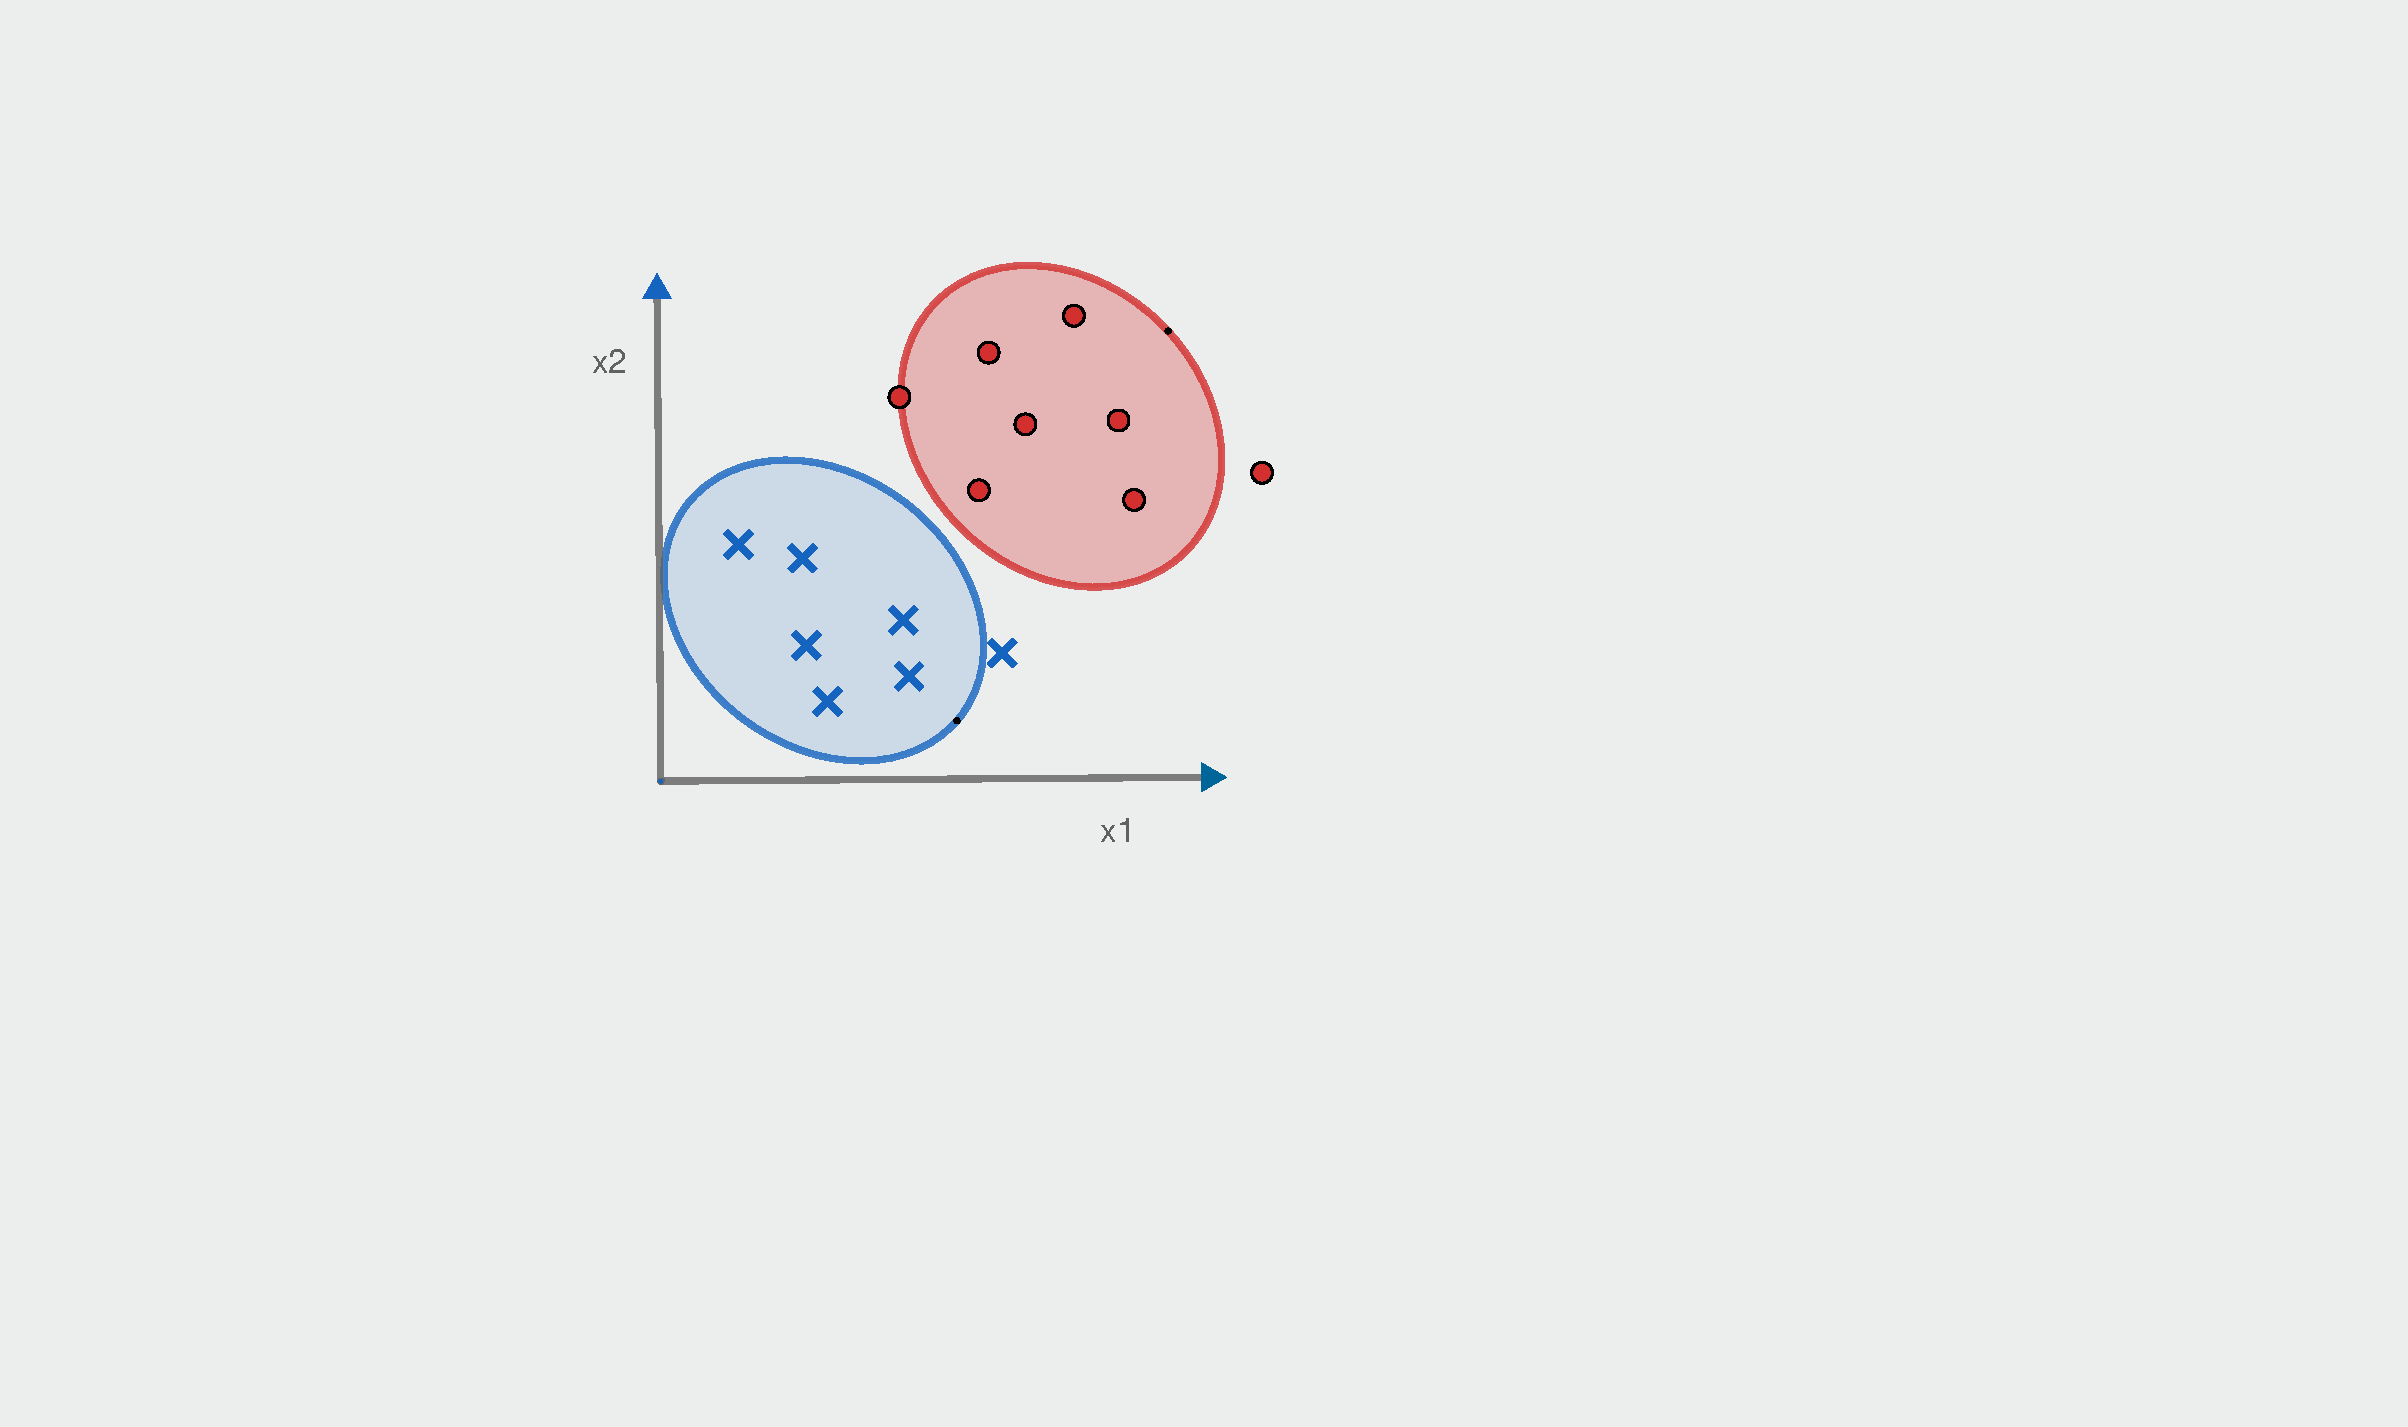
\includegraphics[trim =9.6cm 9.6cm 19cm 4cm, clip = true, totalheight=0.26\textheight]{plots/Images/generative_model.pdf}
		\captionof{figure}{Generative approach.}
		\label{fig:test2}
	\end{minipage}
%\caption{Discriminative and Generative approach.}
\end{figure}
\section{Discriminative modeling}
In this section, we review the basics of discriminative modeling proposed in \cite{HDGEmain}. Given a data distribution through the probability density $p(\boldsymbol{x})$ and a label distribution with probability density $p(y|\boldsymbol{x})$ containing $C$ categories. In other words, the variable $y$ is now categorical, taking on $C$ possible values, and comes from a finite set $\pazocal{C}$.  A classification problem is typically solved using a parametric function $f_{\boldsymbol{\theta}} : \mathbb{R}^D \to \pazocal{C}$, where $\boldsymbol{\theta}$ denotes the parameters of the model. In practice, the function $f_{\boldsymbol{\theta}}$ is often used in the form of $\mathbb{R}^D \to  \mathbb{R}^C$. This function maps each data point $\boldsymbol{x} \in \mathbb{R}^D$ to $C$ real-valued numbers known as logits. It should be noted that $\mathbb{R}^C$ is allowed here due to the utilization of \emph{one-hot encoding}, which will be explained in Section \ref{OHE}. Logits are used to parameterize a categorical distribution through the function.
\begin{equation}\label{softmax}
	q_{\boldsymbol{\theta}}\left(y|\boldsymbol{x}\right) = \frac{\exp\left({f_{\boldsymbol{\theta}}\left(\boldsymbol{x}\right)[y]}\right)}{\sum_{i=1}^C\exp\left({f_{\boldsymbol{\theta}}\left(\boldsymbol{x}\right)[y_i]}\right)},
\end{equation}
which is known as the Softmax function. Note that the convention $f_{\boldsymbol{\theta}}\left(\boldsymbol{x}\right)[y]$ means the element $y^{\mathrm{th}}$ of $f_{\boldsymbol{\theta}}\left(\boldsymbol{x}\right)$. For learning $f_{\boldsymbol{\theta}}$ is usually minimized cross-entropy loss 
\begin{equation}\label{crossentropy}
	\min_{\boldsymbol{\theta}}- \mathbb{E}_{p(y|\bx)}\left[\log q_{\boldsymbol{\theta}}\left(y|\boldsymbol{x}\right)\right].
\end{equation} 
The rationale for this objective comes from minimizing the Kullback-Leibler (KL) divergence with a target distribution $p(y| \boldsymbol{x})$ \cite{KL}. In general, the
KL divergence (or KL distance) from $p(y| \boldsymbol{x})$ to $q_{\boldsymbol{\theta}}\left(y|\boldsymbol{x}\right)$ is defined as
\begin{equation}\label{eq:KLdiv}
D_{\mathrm{KL}} \left(p(y| \boldsymbol{x}) || q_{\boldsymbol{\theta}}\left(y|\boldsymbol{x}\right) \right) = \int p(y| \boldsymbol{x})\log\frac{p(y| \boldsymbol{x})}{q_{\boldsymbol{\theta}}\left(y|\boldsymbol{x}\right)}\d{y} = \mathbb{E}_{p(y| \boldsymbol{x})} \left[\log\frac{p(y| \boldsymbol{x})}{q_{\boldsymbol{\theta}}\left(y|\boldsymbol{x}\right)} \right]
\end{equation}
and has the following properties:
\begin{enumerate}
\item $\KL{p(y| \boldsymbol{x})}{q_{\boldsymbol{\theta}}\left(y|\boldsymbol{x}\right)} \geq 0,$
\item $\KL{p(y| \boldsymbol{x})}{q_{\boldsymbol{\theta}}\left(y|\boldsymbol{x}\right)} = 0$ iff $p(y| \boldsymbol{x}) = q_{\boldsymbol{\theta}}\left(y|\boldsymbol{x}\right)$ almost everywhere,
\item $\KL{p(y| \boldsymbol{x})}{q_{\boldsymbol{\theta}}\left(y|\boldsymbol{x}\right)} \neq \KL{q_{\boldsymbol{\theta}}\left(y|\boldsymbol{x}\right)}{p(y| \boldsymbol{x})}$ and KL divergence does not obey the triangle inequality.
\end{enumerate}
The third property indicates that care is needed in the syntax describing KL divergence. We say that \eqref{eq:KLdiv} is from $p(y| \boldsymbol{x})$ to $q_{\boldsymbol{\theta}}\left(y|\boldsymbol{x}\right)$. Using the logarithmic property, \eqref{eq:KLdiv} can be further rewritten in the form 
\begin{equation}
	 \mathbb{E}_{p(y| \boldsymbol{x})} \left[\log\frac{p(y| \boldsymbol{x})}{q_{\boldsymbol{\theta}}\left(y|\boldsymbol{x}\right)} \right] = 
	 \mathbb{E}_{p(y| \boldsymbol{x})} \left[\log p(y| \boldsymbol{x}) \right] - \mathbb{E}_{p(y| \boldsymbol{x})} \left[\log q_{\boldsymbol{\theta}}\left(y|\boldsymbol{x}\right) \right],
	\end{equation}
where subscript $\boldsymbol{\theta}$ emphasizes that $q_{\boldsymbol{\theta}}\left(y|\boldsymbol{x}\right)$ is the approximative density we get to control. Note that
the first term does not depend on $\bt$ and therefore minimizing either CE or KL divergence is equivalent. Finally, by minimizing with respect to $\bt$ we obtain
\begin{equation}
\min_{\boldsymbol{\theta}} D_{\mathrm{KL}} \left(p(y| \boldsymbol{x}) \Vert q_{\boldsymbol{\theta}}\left(y|\boldsymbol{x}\right) \right) = \min_{\boldsymbol{\theta}} - \E_{p(y| \boldsymbol{x})}\left[ \log q_{\boldsymbol{\theta}}\left(y|\boldsymbol{x}\right)\right].
\end{equation}
For clarity, the expected value will be discussed. In practice, it is dealt with discrete data, so the term $\E_{ p(y| \boldsymbol{x})}\left[\log q_{\boldsymbol{\theta}}\left(y|\boldsymbol{x}\right)\right]$ takes the form of
\begin{equation}
    \E_{p(y| \boldsymbol{x})}\left[\log q_{\boldsymbol{\theta}}\left(y|\boldsymbol{x}\right)\right] = \sum_{k=1}^C p(y_k| \boldsymbol{x})\log q_{\boldsymbol{\theta}}\left(y_k|\boldsymbol{x}\right).
\end{equation}
This part deserves further discussion for a few reasons:
\begin{itemize}
    \item Maximum likelihood estimation (ML) of $\bt$ is equivalent to minimization of the KL distance.
    \item One may encounter the concepts of minimization or maximization of CE.
\end{itemize}
To address the first mentioned reason, it is necessary to break down ML estimation. Since $q_{\boldsymbol{\theta}}\left(y|\boldsymbol{x}\right)$ is the PDF model, we have to follow the objective function.
\begin{equation}
    q_{\boldsymbol{\theta}}\left(y_1,y_2,\dots,y_N|\boldsymbol{x}_1, \bx_2, \dots, \bx_N\right) = \prod_{i=1}^{N}q_{\boldsymbol{\theta}}\left(y_i|\boldsymbol{x_i}\right).
\end{equation}


\subsection{One--hot encoding}\label{OHE}
 Machine learning (ML) algorithms can misinterpret the numeric values of labels if there exists any hierarchy between them. One--hot encoding is a very common approach for dealing with this issue, in order to improve the algorithm performance. Each unique category value is transformed into a new column and these dummy variables are then filled up with 0 or 1 (0 for FALSE and 1 for TRUE). For the sake of clarity, the transformation of a label encoding into a one--hot encoding is illustrated in the following table \ref{tab:OHE}. 
 
 However, this method has its own downsides. For example, it creates new variables and if there exist many unique category values, models have to deal with a large number of predictors, causing the so-called \emph{Big-p problem} \cite{Bigp}. Also, one--hot encoding causes multicolinearity between the individual variables, which may lead to reducing the model's accuracy. 
 \begin{table}[h]
 \centering
 	\begin{tabular}{|l|l|l|}
 		\hline
 		Food Name & Categorical \# & Calories \\ \hline
 		Pizza     & 1              & 266      \\ \hline
 		Hamburger & 2              & 295      \\ \hline
 		Caviar    & 3              & 264      \\ \hline
 	\end{tabular}
 	\quad $\Rightarrow$ \quad
	\begin{tabular}{|l|l|l|l|}
		\hline
		Pizza & Hamburger & Caviar & Calories \\ \hline
		1     & 0         & 0      & 266      \\ \hline
		0     & 1         & 0      & 295      \\ \hline
		0     & 0         & 1      & 264      \\ \hline
	\end{tabular}
	\caption{Transformation of a label encoding (left) to the one--hot encoding (right).}
	\label{tab:OHE}
 \end{table}
\section{Generative modeling}

\subsection{Variational autoencoder}
The first generative modeling approach that will be discussed is the variational autoencoder (VAE). In this section, motivation will be addressed and individual mathematical aspects will be discussed in detail. 
\subsubsection{Problem scenario}
Assume that the data $\boldsymbol{X}=\left\lbrace x_i \right\rbrace^N_{i=1}$ are generated by some random process involving an unobserved continuous variable $\boldsymbol{z}$, which will be referenced as a latent variable or code. The objective is again to find the PDF of the given data in parametric form $p_{\bt}\left(\bx\right)$. One can choose an approximative distribution in the form of
\begin{equation}\label{eq:VAE_approxform}
p_{\bt}\left(\bx\right) = \int p_{\bt}\left(\bx,  \boldsymbol{z}\right)\d{\boldsymbol{z}} =\int p_{\bt}\left(\bx\vert \boldsymbol{z}\right)p_{\bt}\left(\boldsymbol{z}\right)\d{\boldsymbol{z}},
\end{equation}
But such an approximation is usually very expensive to compute or can even be intractable. Intractability of the $p_{\bt}\left(\bx\right)$ makes posterior PDF $p_{\bt}\left(\boldsymbol{z}\vert\bx\right)$ also intractable.

\subsubsection{Naive approach}
One of the simplest ways to solve this problem may seem to be to build a model depending on the latent variable $f_{\bt}\left(\boldsymbol{z}\right)$ and try to train its parameters. For simplicity, let $p\left(\boldsymbol{z} \right) = \pazocal{N}\left(\boldsymbol{0}, \mathbb{I}_P\right)$, where $P$ denotes the dimension of the latent space $\boldsymbol{z}$ and also let
\begin{equation}
\bx = f_{\bt}\left(\boldsymbol{z}\right) + \boldsymbol{\varepsilon}, \quad \boldsymbol{\varepsilon} \sim \pazocal{N}\left(\boldsymbol{0},\sigma^2\cdot\mathbb{I}_D \right)
\end{equation}
which actually gives 
\begin{equation}\label{eq:VAE_decoder}
p_{\bt}\left(\bx\vert\boldsymbol{z}\right) = \pazocal{N}\left(\boldsymbol{x};f_{\bt}\left(\boldsymbol{z}\right),\sigma^2\cdot\mathbb{I}_D \right).
\end{equation}
It may be noted that the subscript $D$ is the dimension of the data point $\bx$. The true PDF of the given data can be cleverly written using the empirical PDF, i.e., in the form of $p_{\mathrm{emp}}\left(\boldsymbol{x} \right)~=~\frac{1}{N}\sum_{i=1}^N\delta\left(\bx - \bx_i\right) $,
which can be exploited by finding the $\bt$ parameters by minimizing the $\KL{p_{\mathrm{emp}}\left(\boldsymbol{x} \right)}{p_{\bt}\left(\bx\right)}$. Since minimizing the KL distance is equivalent to ML estimation and using the approximative form \eqref{eq:VAE_approxform}, the following holds 
\begin{align}
    \widehat{\boldsymbol{\bt}} &= \argmin_{\boldsymbol{\bt}}- \sum_{i=1}^N\log p_{\boldsymbol{\bt}}\left(\boldsymbol{x}_i \right)\\
    &=  \argmin_{\boldsymbol{\bt}}- \sum_{i=1}^N \log \int \pazocal{N}\left(\boldsymbol{x}_i;f_{\bt}\left(\boldsymbol{z}\right),\sigma^2\cdot\mathbb{I}_D \right) \cdot \pazocal{N}\left(\boldsymbol{z};\boldsymbol{0}, \mathbb{I}_P\right) \d{\boldsymbol{z}}\\
    &= \argmin_{\boldsymbol{\bt}}- \sum_{i=1}^N \log \sum_{j=1}^{P}\exp\left(-\frac{1}{2\sigma^2}\left(\bx_i-f_{\bt}\left(\boldsymbol{z}_j\right)\right)^\top\left(\bx_i-f_{\bt}\left(\boldsymbol{z}_j\right)\right) \right).
\end{align}
Integration over $\boldsymbol{z}$ is represented by sampling. In iterations, for an incorrect value of $\bt$, all the generated samples may
be away from the samples of $\boldsymbol{x}$, and the gradient is poor.


\subsubsection{Variational Bayes approach}
\begin{figure}[h]
	\centering
	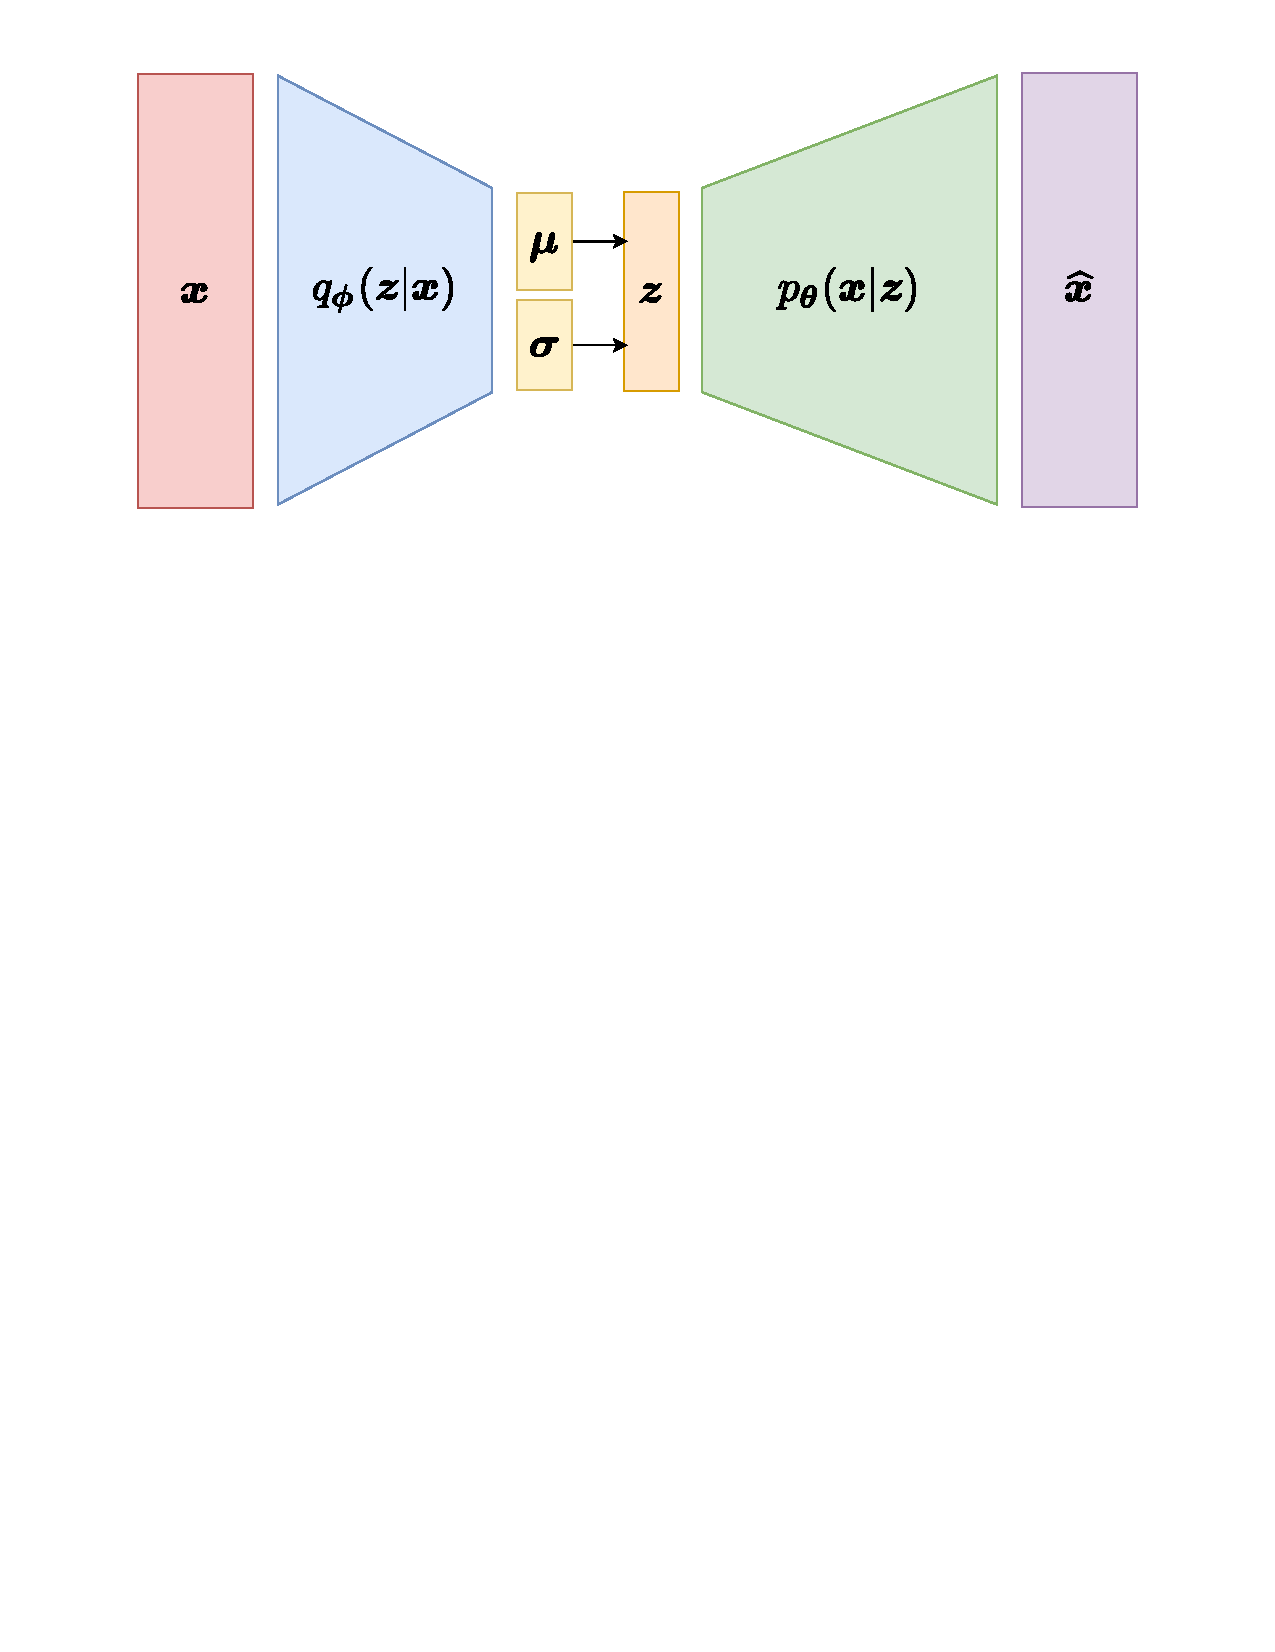
\includegraphics[width=\textwidth, trim={0 19cm 0 0cm}]{plots/Images/VAE_diagram.pdf}
	\caption{VAE diagram.}%
	\label{fig:VAE_architecture}%
\end{figure}

To solve this problem, it is necessary to introduce a further approximative posterior distribution $q_{\bphi}\left(\boldsymbol{z}\vert\bx\right) \approx p_{\bt}\left(\boldsymbol{z}\vert\bx\right)$ with parameters $\bphi$, preferably Gaussian. Standard terminology refers to the model $q_{\bphi}\left(\boldsymbol{z}\vert\bx\right)$ as a probabilistic \emph{encoder} and  $p_{\bt}\left(\bx\vert \boldsymbol{z}\right)$ is called a probabilistic \emph{decoder}. For VAE, the idea is to use the KL distance from $q_{\bphi}\left(\boldsymbol{z}\vert\bx\right)$ to $p_{\bt}\left(\boldsymbol{z}\vert \bx\right)$, which produces
\begin{equation}\label{eq:VAEloss}
\begin{split}
D_{\mathrm{KL}}\left(q_{\bphi}\left(\boldsymbol{z}\vert \bx \right) \Vert p_{\bt}\left(\boldsymbol{z}\vert \bx\right)\right) & = 
\int q_{\bphi}\left(\boldsymbol{z}\vert \bx \right) \log \frac{q_{\bphi}\left(\boldsymbol{z}\vert \bx \right)}{p_{\bt}\left(\boldsymbol{z}\vert \bx\right)} \d{\boldsymbol{z}} \\
& =  \int q_{\bphi}\left(\boldsymbol{z}\vert \bx \right) \log \frac{q_{\bphi}\left(\boldsymbol{z}\vert \bx \right)p_{\bt}\left(\bx\right)}{p_{\bt}\left(\bx \vert \boldsymbol{z}\right) p_{\bt}\left(\boldsymbol{z}\right)} \d{\boldsymbol{z}} \\
& = \log p_{\bt}\left(\boldsymbol{x}\right) +  \int q_{\bphi}\left(\boldsymbol{z}\vert \bx \right) \log \frac{q_{\bphi}\left(\boldsymbol{z}\vert \bx \right)}{p_{\bt}\left(\bx \vert \boldsymbol{z}\right)p_{\bt}\left(\boldsymbol{z}\right) } \d{\boldsymbol{z}} \\
& = \log p_{\bt}\left(\boldsymbol{x}\right) +  \mathbb{E}_{q_{\bphi}\left(\boldsymbol{z}\vert \bx \right)}\left[\log\frac{q_{\bphi}\left(\boldsymbol{z}\vert \bx \right)}{p_{\bt}\left(\boldsymbol{z}\right)} - \log p\left(\textbf{x}\vert \boldsymbol{z}\right)\right]\\
    & = \log p_{\bt}\left(\boldsymbol{x}\right) +\KL{q_{\bphi}\left(\boldsymbol{z}\vert \bx \right)}{p_{\bt}\left(\boldsymbol{z}\right)} -  \mathbb{E}_{q_{\bphi}\left(\boldsymbol{z}\vert \bx \right)}\left[\log p\left(\bx\vert \boldsymbol{z}\right)\right].
 \end{split}
\end{equation}
Using the last equality of \eqref{eq:VAEloss}, it is possible to rewrite the equation in its typical form
\begin{equation}
\log p_{\bt}\left(\bx\right) - D_{\mathrm{KL}}\left(q_{\bphi}\left(\boldsymbol{z}\vert \bx \right) \Vert p_{\bt}(\boldsymbol{z}\vert \bx)\right) = \underbrace{\mathbb{E}_{q_{\bphi}\left(\boldsymbol{z}\vert \bx \right)}\left[\log p_{\bt}(\bx\vert \boldsymbol{z}) \right] - D_{\mathrm{KL}}\left(q_{\bphi}\left(\boldsymbol{z}\vert\bx \right) \Vert p_{\bt}\left(\boldsymbol{z}\right)\right)}_{\text{= $L\left(\bt,\bphi; \bx\right)$}},
\end{equation}
where the right-hand side is called \emph{variational lower bound}. There is no uniformity in terminology, and thus one can also encounter the name evidence lower bound (ELBO). The first term on the right-hand side is known as reconstruction loss, and the second term is often called a regularization term. As a KL distance is always non-negative, it holds
\begin{equation}
    \log p_{\bt}\left(\bx\right) \geq L\left(\bt,\bphi; \bx\right).
\end{equation}
The objective is to maximize the log-likelihood $\log p_{\bt}\left(\bx\right)$ which is equivalent to minimizing the negative log-likelihood and that is what will be used here. At this point, we have a lower bound for one data point $\bx$, but we need to include all observations in the lower bound. The joint log-likelihood can be rewritten as a sum over the marginal log-likelihoods of individual observations $\log p_{\bt}\left(\bx_1,\bx_2,\dots,\bx_N\right)~=~\sum_{i=1}^N\log p_{\bt}\left(\bx_i\right)$ that completes all the building blocks needed to determine the optimization equation. This formulation provides one major advantage, which is that it is now possible to jointly optimize both the generative parameters $\bt$ and the variational parameters $\bphi$ as follows 
\begin{align}
   \widehat{\bt}, \widehat{\bphi} &= \argmin_{\bt,\bphi}-\sum_{i=1}^N\log p_{\bt}\left(\bx_i\right)\\
   &=\argmin_{\bt,\bphi}-\sum_{i=1}^N L\left(\bt,\bphi; \bx_i\right)\\
  &= \argmin_{\bt,\bphi}-\sum_{i=1}^N\mathbb{E}_{q_{\bphi}\left(\boldsymbol{z}\vert \bx_i \right)}\left[\log p_{\bt}(\bx_i\vert \boldsymbol{z}) \right] - D_{\mathrm{KL}}\left(q_{\bphi}\left(\boldsymbol{z}\vert\bx_i \right) \Vert p_{\bt}\left(\boldsymbol{z}\right)\right).\label{eq:VAEloss}
\end{align}
For a better understanding of the problem, a VAE diagram is shown in Figure \ref{fig:VAE_architecture}. Note that the latent space is usually much smaller than the input space, and for this reason, it is also sometimes called the bottleneck. 


\subsubsection{Reparameterization trick}
\begin{wrapfigure}{r}{0.45\textwidth}
  \begin{center}
    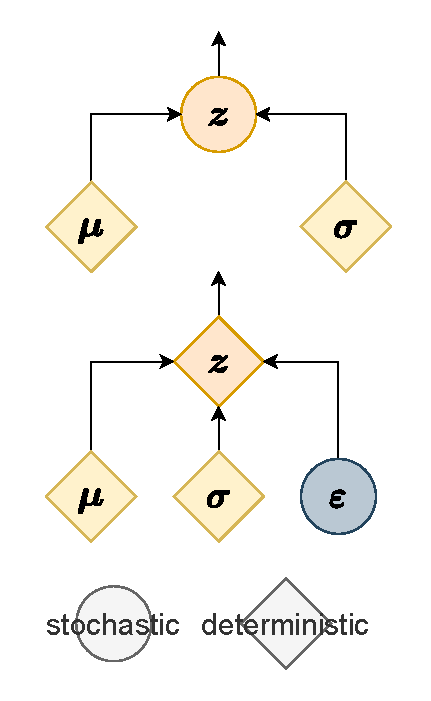
\includegraphics[trim={3cm 1.4cm 3cm 2.6cm}]{plots/Images/reparam_resized.pdf}
  \end{center}
  	\caption{Reparametrization trick.}%
	\label{fig:VAE_reparam}%
\end{wrapfigure}
The key success of VAE lies in the fact that \eqref{eq:VAEloss} can be efficiently computed using \emph{reparameterization trick}, where we express $\boldsymbol{z}$ as a deterministic variable
\begin{equation}\label{eq:reparam_general}
\boldsymbol{z} = g_{\bphi}\left(\boldsymbol{\varepsilon},\bx\right),
\end{equation}
 where $\boldsymbol{\varepsilon}$ stands for an auxiliary variable with independent marginal $p\left(\boldsymbol{\varepsilon}\right)$ and $g_{\bphi}\left(.\right)$ is a function parameterized by $\bphi$. 

A common explanation for this trick is that during the optimization the gradient cannot back--propagate through a random node. So, in the case of VAE, the reparameterization trick shifts the source of randomness to another variable different from $\boldsymbol{z}$ and allows differentiation with respect to $\boldsymbol{z}$. However, this explanation may not be sufficient and for this reason we will state a more formal justification. Consider taking the gradient with respect to $\bt$ of $\mathbb{E}_{p(\bz)}\left[\model{z} \right]$. It can be easily computed as
\begin{align}
    \nabla_{\bt}  \mathbb{E}_{p(\bz)}\left[\model{z} \right] &= \nabla_{\bt} \int p(\bz) \model{z} \d{\bz} \\
    &= \int p(\bz) \nabla_{\bt} \model{z} \d{\bz} \\
    &=  \mathbb{E}_{p(\bz)}\left[\nabla_{\bt}\model{z} \right].\label{eq:nonparametricexpectation}
\end{align}
The result is obvious; the gradient of the expectation is equal to the expectation of the gradient. However, the gradient of the expectation becomes much more interesting if the PDF $p_{\bt}(\bz)$ is also parameterized by $\bt$, resulting in 
\begin{align}
    \nabla_{\bt}  \mathbb{E}_{p_{\bt}(\bz)}\left[\model{z} \right] &= \nabla_{\bt} \int p_{\bt}(\bz) \model{z} \d{\bz} \\
    &= \int p_{\bt}(\bz) \nabla_{\bt} \model{z} \d{\bz} + \int  \model{z} \nabla_{\bt}p_{\bt}(\bz)\d{\bz} \\
    &=  \mathbb{E}_{p_{\bt}(\bz)}\left[\nabla_{\bt}\model{z} \right] + \int  \model{z} \nabla_{\bt}p_{\bt}(\bz)\d{\bz}. \label{eq:paramexpectation}
\end{align}
The second term of \eqref{eq:paramexpectation} is not guaranteed to be an expectation and this very fact indicates that backpropagation would not compute an estimate of $\nabla_{\bt}  \mathbb{E}_{p_{\bt}(\bz)}\left[\model{z} \right]$. That being the case, if we apply the reparameterization trick $\bz =g_{\bt}\left(\boldsymbol{\varepsilon},\bx\right)$ to this simple example, we get
\begin{equation}
\mathbb{E}_{p_{\bt}(\bz)}\left[\model{z} \right] = \mathbb{E}_{p(\boldsymbol{\varepsilon})}\left[f\left(g_{\bt}(\boldsymbol{\varepsilon}, \bx)\right) \right].
\end{equation}
At this point, it is possible to take the gradient $\nabla_{\bt} \mathbb{E}_{p(\boldsymbol{\varepsilon})}\left[f\left(g_{\bt}(\boldsymbol{\varepsilon}, \bx)\right) \right]$ analogously to that in \eqref{eq:nonparametricexpectation}. To be perfectly clear, the authors of [] proposed an easy exercise. Take the univariate Gaussian case $p(z|x) = \pazocal{N}\left(\mu, \sigma^2\right)$. In such a case, proper reparametrization takes the shape of
\begin{equation}\label{eq:VAE_reparam1D}
z = \mu + \sigma\varepsilon,
\end{equation}
where $\varepsilon\sim\pazocal{N}\left(0,1\right)$ and, therefore, the expectation
\begin{equation}
    \mathbb{E}_{\pazocal{N}\left(z;\mu, \sigma^2\right)}\left[f(z)\right] = \mathbb{E}_{\pazocal{N}\left(\varepsilon;0, 1\right)}\left[f(\mu + \sigma\varepsilon)\right] \approx \frac{1}{M}\sum_{j=1}^M f\left(\mu + \sigma\varepsilon_j\right).
\end{equation}
Note that this is nothing more than a transformation of a random variable. And this is exactly the problem with optimizing ELBO \eqref{eq:VAEloss}. We need to rewrite the expectation $\mathbb{E}_{q_{\bphi}\left(\boldsymbol{z}\vert\bx_i \right)}$ so that the Monte Carlo estimate of the expected value is differentiable with respect to $\boldsymbol{\phi}$.

\subsubsection{Variational autoencoder}
So far we have only dealt with VAE in general. In this section, we put everything together and specify the individual parts of the ELBO \eqref{eq:VAEloss}.
Let the probabilistic encoder be a multivariate Gaussian with a diagonal covariance matrix
\begin{equation}\label{eq:VAE_q}
q_{\bphi}\left(\boldsymbol{z}\vert \bx \right) = \pazocal{N}\left(\boldsymbol{z}; \boldsymbol{\mu},\boldsymbol{\sigma}^2\mathbb{I}_P  \right) 
\end{equation}
and let the probabilistic decoder takes the form depending on the type of given data and model.This is typically either multivariate Gaussian or Bernoulli. Finally, let the prior $p_{\bt}\left(\bz\right)$ be the centered izotropic multivariate Gaussian, i.e.
\begin{equation}
p_{\bt}\left(\boldsymbol{z} \right) = p\left(\boldsymbol{z} \right) = \pazocal{N}\left(\boldsymbol{z}; \boldsymbol{0},\mathbb{I}_P  \right),
\end{equation}
where the generative parameters $\bt$ are omitted, since the chosen prior distribution lacks parameters. When using \eqref{eq:VAE_q}, $\boldsymbol{\mu}$ and $\boldsymbol{\sigma}$ are non-linear functions of the data point $\bx$ and the variational parameters $\bphi$. This setting actually allows us to take the reparameterization trick in a form similar to that of Equation \eqref{eq:VAE_reparam1D}, which means that
\begin{equation}\label{eq:reparam_specific}
\boldsymbol{z}_{i,j} = \boldsymbol{\mu}_i + \boldsymbol{\sigma}_i\odot\boldsymbol{\varepsilon}_j ,
\end{equation}
where the symbol $\odot$ denotes the Hadamard product, i.e., the element-wise product and the auxiliary variable $\boldsymbol{\varepsilon} \sim \pazocal{N}\left(\boldsymbol{0},\mathbb{I} \right)$.
Another important fact is that the KL distance from a Gaussian distribution to a Gaussian distribution has an analytical solution, so $\KL{q_{\bphi}\left(\bz\vert \bx \right)}{p_{\bt}\left(\bz\right)}$ can be expressed in closed form:
\begin{equation}
\begin{split}
 \KL{q_{\bphi}\left(\bz\vert \bx \right)}{p_{\bt}\left(\bz\right)} & = \KL{\pazocal{N}\left(\boldsymbol{z}; \boldsymbol{\mu},\boldsymbol{\sigma}^2\mathbb{I}_P  \right) }{\pazocal{N}\left(\boldsymbol{z}; \boldsymbol{0},\mathbb{I}_P  \right)}\\ & =\frac{1}{2}\sum_{j=1}^P\left(1 + \log\sigma^2_j -\mu_j^2 -\sigma_j^2 \right).
\end{split}
\end{equation}
Now all that is left is to plug everything into equation \eqref{eq:VAEloss}, which leads to the final form
\begin{align}\label{řešení_VAE}
 \widehat{\bt}, \widehat{\bphi} & = \argmin_{\bt,\bphi}-\sum_{i=1}^N\mathbb{E}_{q_{\bphi}\left(\boldsymbol{z}\vert \bx_i \right)}\left[\log p_{\bt}(\bx_i\vert \boldsymbol{z}) \right] - D_{\mathrm{KL}}\left(q_{\bphi}\left(\boldsymbol{z}\vert\bx_i \right) \Vert p_{\bt}\left(\boldsymbol{z}\right)\right) \\
 & = \argmin_{\bt, \bphi}-\sum_{i = 1}^N\left(\frac{1}{P}\sum_{j = 1}^P \log p_{\bt}\left(\bx_i\vert \bz_{i,j}\right) +   \frac{1}{2}\sum_{j=1}^P\left(1 + \log\sigma^2_{i,j} -\mu_{i,j}^2 -\sigma_{i,j}^2 \right)\right).
\end{align}



\subsection{Noise--contrastive estimation}
Suppose one has to estimate a model that is specified by an nonnormalized probability density function $q^0_{\bt}\left(\boldsymbol{x}\right)$. In such a case, one can utilize noise--contrastive estimation (NCE). The first step is to introduce another parameter $c$ among the estimated parameters $\bt$. For clarity, the symbol $\bt^\star=\left\lbrace\bt,c\right\rbrace$ is introduced for the set of estimated parameters, including
$c$. Using this notation, the following equalities hold
\begin{align}
    q_{\bt^\star}\left(\boldsymbol{x}\right)
    \end{align}
which means that the newly introduced parameter $c$ is an estimate of the negative logarithm of
the normalization constant $Z\left(\bt\right)$.
As the name suggests, we use noise to estimate. By our convention, let $\bx_1,\bx_2,\dots,\bx_N$
be the observations and $\boldsymbol{e}_1,\boldsymbol{e}_2,\dots,\boldsymbol{e}_N$ be the artificially generated noise data with known distribution $\psi\left(\bt\right)$. The estimate $\widehat{\bt^\star}$ is then defined as
\begin{align}
    \widehat{\bt^\star} &= \argmax_{\bt^\star} \pazocal{L}^{\mathrm{NC}}\left(\bt^\star\right)\\
   &= \argmax_{\bt^\star} \frac{1}{2N}\sum_{i=1}^N \ln\sigma_{\bt^\star}\left(\bx_i\right) + \ln\left(1-\sigma_{\bt^\star}\left(\boldsymbol{e}_i\right) \right)\label{NCEloss}
\end{align}
where $\sigma_{\bt^\star}$ is a logistic function,
\begin{align}
\sigma_{\bt^\star} = \frac{1}{1 + \exp\left(-G_{\bt^\star}\left(\bx\right) \right)}
\end{align}
and finally, the function $G_{\bt^\star}$ represents the difference of the log-likelihoods of $q_{\bt^\star}$ and $\psi$, hence the
\begin{align}
    G_{\bt^\star} = \ln q_{\bt^\star}\left(\bx \right) - \ln\psi\left(\bx \right).
\end{align}
It may be noted that equation \eqref{NCEloss} also appears in SL tasks and is called binary
CE loss. It is actually a special case of CE itself. Thus, it is used for the classification of two classes. This gives an intuitive insight into how noise--contrastive estimation
really works. When data and noise are compared, the model is learned, so this method can be called
learning by comparison. This approach does not use labels, so it is a UL algorithm. 
\begin{example}[Gaussian distribution]
To test this approach, we performed a simple experiment. There are a total of $N = 100$ i.i.d. one-dimensional observations $x_1,x_2,\dots,x_N$ from an unknown distribution that is assumed to be nonnormalized and Gaussian. Therefore, it is of the form
\begin{align}
    q_{\bt^\star}\left(x\right) = \exp\left(-\frac{1}{2}\cdot\frac{\left(x-\mu\right)^2}{\sigma^2} + c \right)
\end{align}
where $\bt^\star = \left\lbrace \mu, \sigma^2, c \right\rbrace$. Next, we artificially generate $N = 100$ noise data $e_1,e_2,\dots,e_N$, which is again easier to do using a Gaussian distribution. This means that it can be chosen, for example,
\begin{align}
    \psi\left(e\right) = \frac{1}{\sqrt{2\pi 10}}\exp\left(-\frac{1}{2}\cdot\frac{e^2}{10} \right)
\end{align}
At this point, it is possible to construct a function $\pazocal{L}^{\mathrm{NC}}\left(\bt^\star\right)$ that is minimized by using stochastic
gradient descent. The following figure shows the training process and the comparison between
the estimated distribution and the true one. As can be seen in Figure 4.1, this approach works quite well and for more observations the results would be even better.
\begin{figure}[h]
	\centering
	\subfloat[Training loss function]
	{{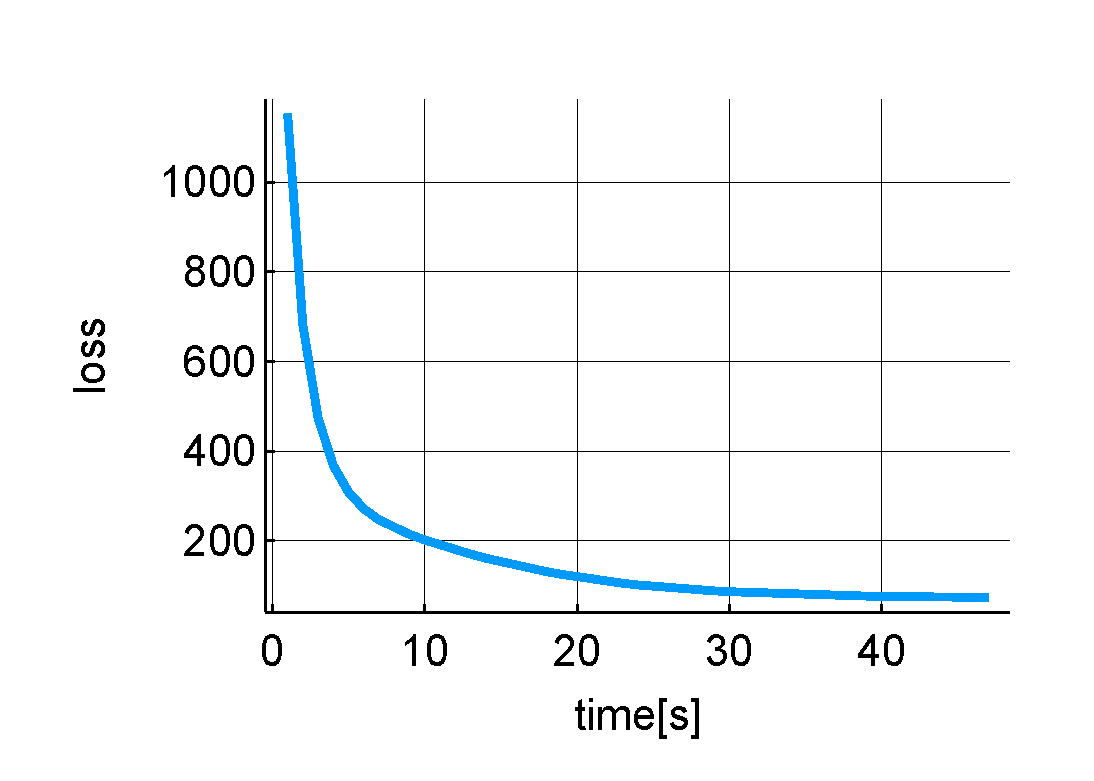
\includegraphics[width=8.0cm]{plots/Images/NCE_loss} }}%
	\subfloat[Comparison of true and estimated pdf]
	{{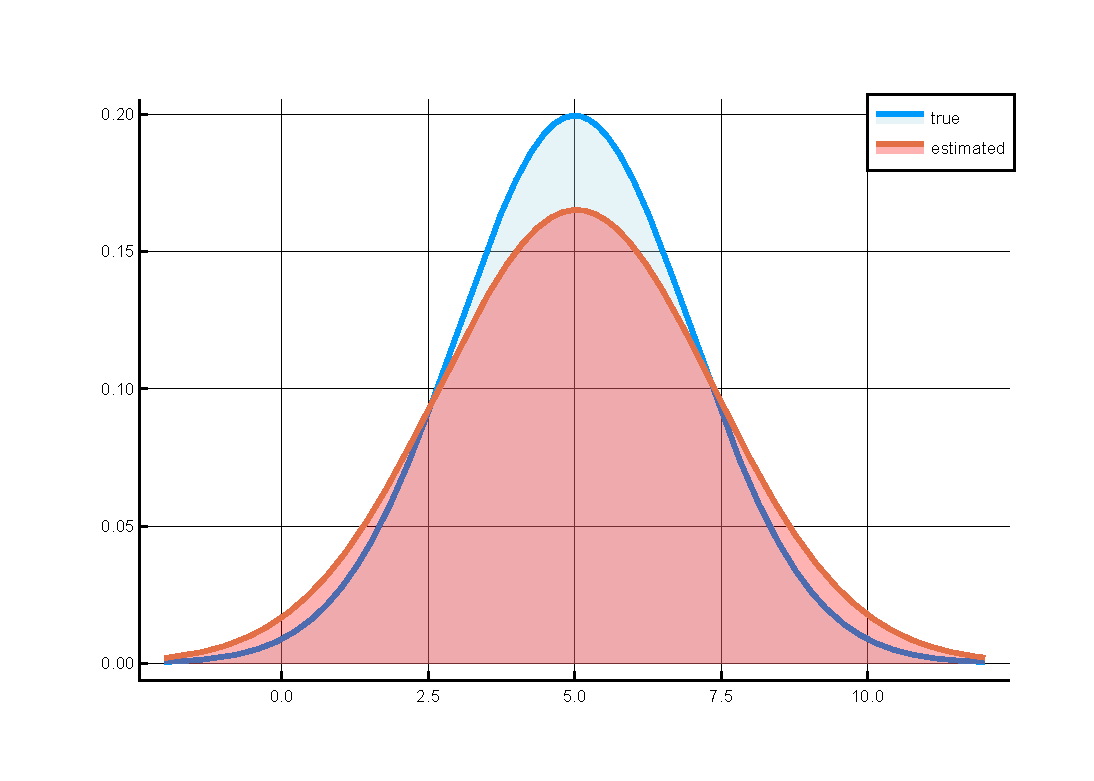
\includegraphics[width=8.0cm]{plots/Images/NCE_results.pdf} }}%
	\caption{Results of the NCE experiment}%
	\label{ggm}%
\end{figure}
\end{example}